\chapter{Introduction}
\label{cha:introduction}

% the code below specifies where the figures are stored
\ifpdf
    \graphicspath{{1_introduction/figures/PNG/}{1_introduction/figures/PDF/}{1_introduction/figures/}}
\else
    \graphicspath{{1_introduction/figures/EPS/}{1_introduction/figures/}}
\fi

\section{Motivation and Problem Statement}

A~very open definition of the word \emph{event}
given by WordNet~\cite{fellbaum1998wordnet,miller1995wordnet} is
\emph{``something that happens at a~given place and time''}.
Following this definition,
we are indeed surrounded by events, most of them
are of little to no interest for us.
A~concert somewhere in the world of a~band
that we do not even know may be a~good example.
For some events, however, we may care more, for example,
a~concert of a~band that we know and like,
even if it takes place at a~location far away from us.
Finally, for very few events, we may care a~lot,
maybe even enough to physically attend the event,
like a~concert of our favorite band
if it takes place in our city, is not sold out,
and not too expensive.

All this motivates the need for \emph{event summarization}.
If there is an event that we could not attend
for a~reason whatsoever,
but that we are interested in,
a~good event summarization can help us get a~feeling
for the event's atmosphere.
Similarly, if there is an event that we attended,
we can revive the event's most fascinating moments
based on the event summarization.

A~\emph{media gallery} in the context of
our event summarization task is
a~compilation of images, videos,
and microposts retrieved from social networks
that are related to a~given event.
High quality media galleries have the following properties:

\begin{enumerate}
  \item \textit{Conciseness:}
        they convey a~lot of information clearly
        and in few media items.
  \item \textit{Comprehensiveness:}
        they are complete, including all representative
        elements or aspects of an event.
  \item \textit{Authenticity:}
        they are of undisputed origin and genuine.
  \item \textit{Diversity:}
        they show a~great deal of variety.
  \item \textit{Interestingness:}
        they catch and hold the attention of the viewer.     
\end{enumerate}

Event summarization covers textual,
as well as multimedia content.
For bigger events, official TV or newspaper journalists
report on site, and oftentimes the event organizers themselves
share official media material,
or even an official press package with event reports and images.

\section{Research Question and Hypothesis}

The main research question for this thesis
can be formulated as follows.
 
\noindent \textit{``Can user-customizable
media galleries that summarize given events be
created solely based on textual and multimedia data
from social networks?''}

\noindent The hypothesis that we test in this thesis
can be formulated as follows.

\noindent \textit{We argue that
through media galleries that leverage content
shared on social networks
a~more \emph{authentic}, more \emph{concise},
more \emph{comprehensive}, more \emph{diverse},
and also more \emph{interesting}
view on events gets possible than by limiting oneself
to officially produced media content;
and that further such media galleries can be generated
more \emph{efficiently} and \emph{in shorter time}
than the officially produced ones.}

\noindent We validate these subjective and objective
criteria with experiments for events of different categories
such as sports, politics, culture, leisure,
music, conferences, \emph{etc.}

\section{Approach}

The objective of this thesis is the development
of methods for the automatic summarization of events
based on media items shared on social networks.
A~schematic overview of the approach can be seen
in~\autoref{fig:thesis-diagram}.
As an event takes places and shortly thereafter
(symbolized by the timeline marked with \emph{2h Event}),
people share media items related to the event
on multiple social networks
(symbolized by the photo and video pictograms
above the event timeline).
Via the textual search functionality of those
different social networks,
we retrieve a~list of potentially event-relevant
microposts that either contain media items directly,
or that provide links to media items
on external media item hosting platforms.
Using third party NLP tools,
we recognize and disambiguate named entities
in the microposts to predetermine their relevancy.
We extract the binary media item data
from social networks or media item hosting platforms
and relate it to the originating microposts
(symbolized by the central cloud).
Using CBIR and CBVR techniques, we first deduplicate
exact and near duplicate media items,
and then cluster similar media items
(symbolized by the green, red, and orange markers).
We rank the deduplicated and clustered list
of media items and their related microposts
according to well-defined ranking criteria.
In order to to generate interactively user-customizable
media galleries that visually and audibly summarize the
event in question, we compile the top-$n$ ranked
media items and microposts in an aesthetic way
(symbolized by the timeline marked with \emph{5min Summary}).

\begin{figure}[h!]
  \centering
  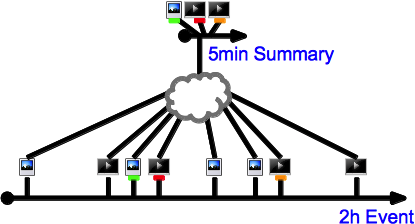
\includegraphics[width=0.5\textwidth]{thesis-diagram.png}
  \caption{Schematic depiction of event summary generation
    based on deduplicated, clustered, and ranked media items
    for an exemplary event.}
  \label{fig:thesis-diagram}
\end{figure}

\section{Contributions}

In this thesis, we report on methods for the automatic generation
of event summaries. Contributions include the following methods.

\begin{itemize}
  \item Methods for named entity extraction and disambiguation
        for online videos based on closed captions.
        \todo{SemWebVid citation}
  \item An examination of Linked Data usage and visualization
        techniques of a~major commercial search engine.
        \todo{How Google is using citation}
  \item The development of a~W3C specification of media
        fragment addressing schemes for audio and video items.
        \todo{Media Fragments citation}
  \item Methods for the semantic description of Web APIs,
        their discovery, consumption, interlinking,
        and social aspects.
        \todo{RESTdesc citations}
  \item A~study of the feasibility of truly RESTful behavior
        for Web APIs in the sense of Dr. Roy Fielding.
        \todo{Fulfilling the hypermedia constraint citation}
  \item The definition of a~unified framework for the description
        of multimedia content objects.
        \todo{Introducing a~unified framework citation}
  \item Methods for the aggregation of social media contents
        for the enhancement of conference experiences.
        \todo{Confomaton citations}
  \item A~study on the usefulness and relevancy of social network
        updates added to the search engine results pages of a~major
        commercial search engine.
        \todo{Adding realtime coverage citation}
  \item An examination of context-aware querying for multimodal
        search engines.
        \todo{Context-aware querying citation}
  \item Methods for the consumer-oriented detection of trending
        microposts on a~major commercial social network.
        \todo{A~tweet consumers' look citation}
  \item Methods for the crowdsourced detection of events in
        online videos.
        \todo{Crowdsourcing event detection citation}
  \item Methods for the definition of aesthetic principles
        for automatic media gallery layout for visual
        and audial event summarization based on social networks.
        \todo{Defining aesthetic principles citation}
  \item An examination of user interface feasibility on
        mobile and desktop devices for a~multimodal search engine.
        \todo{One size does not fit all citation}
  \item Methods for the crowdsourced extraction of knowledge items
        from arbitrary Web pages.
        \todo{SEKI@home citations}
  \item Methods for adding meaning to social network microposts
        via multiple named entity disambiguation APIs and
        tracking their data provenance.
        \todo{Adding Meaning to Social Network citations}
  \item Methods for the automatic extraction of media items from
        multiple social networks.
        \todo{What fresh media citation}
  \item Methods for on-the-fly shot boundary detection of
        online videos.
        \todo{Enabling on-the-fly citation}
   \item Methods for unobtrusively fixing common annoyances on
         arbitrary Web pages.
         \todo{xkcd citation}
   \item A~white paper on future media Internet architecture.
         \todo{FMIA citation}
\end{itemize}

\section{Thesis Structure}

The remainder of this thesis is structured as follows. 
\todo{Add thesis structure}

Each chapter is accompanied by a~final section named
\emph{Chapter Notes}, which contains references of publications
the chapter is (partly) based upon,
and pointers to related material for further reading.